\chapter{Implementation}



\section{Environment}

The software developed in this thesis is completely realized using the Python programming language. This choice was made because OpenStack offers clients that connect to their API and the Elastic Media Manager is also programmed in Python.

PyCharm was selected as the integrated development environment (IDE) to simplify the programming and testing lifecycles. The code is under revision control using git and the repository that contains both the code for the CM and CM Agent consists of two main branches: master and develop. The develop branch holds the latest changes and upon successful testing those were merged back into master, which is always in a production-ready state.


\subsubsection{Project structure}

The code is separated into two different projects in order to allow testing of the integration concurrently. The following graphic outlines the focus within the Elastic Media Manager (EMM), whilst the CM Agent is separated and has its own structure.

\begin{figure}[H]
\centering

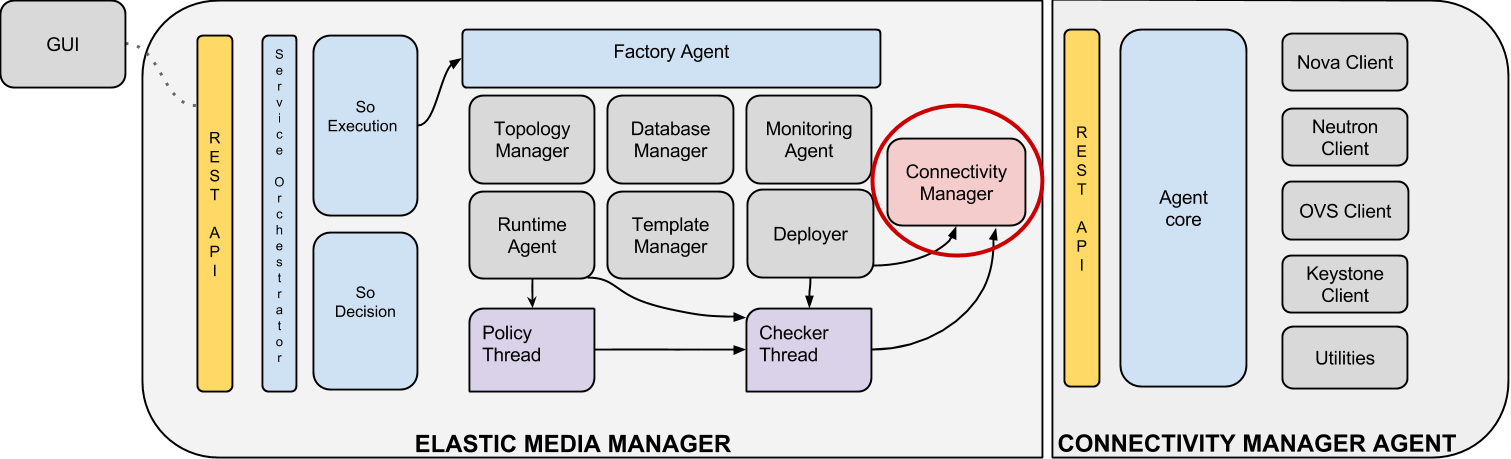
\includegraphics[width=0.7\textwidth]{images/implementation/cm_implementation_focus_overview}

\caption{Implementation focus}
\end{figure}

The structure for the CM is dictated by the already existing implementation of the EMM and the scope of this thesis includes solely its extension with a Connectivity Manager interface and service plus the needed changes in the other interfaces to make use of the methods within the CM.

The Connectivity Manager contains the ReST API, the Agent core, clients and other helper classes.

\subsubsection{Local OpenStack test environment}

In order to test the Connectivity Manager Agent and the use of its OpenStack API clients a testbed was installed. This test-bed was set up using Vagrant, as it allows to start virtual machines from the command-line and can easily be provisioned and managed. In order to test the software across multiple compute nodes a set up with 2 VM's was installed.

For the installation of OpenStack the devstack script was used, which takes care of not only the deployment of the different components but also their configuration. The configuration parameters are set in the 'local.conf' file. For the OpenStack cluster controller the following configuration was used:

\begin{lstlisting}
[[local|localrc]]
ADMIN_PASSWORD=pass
DATABASE_PASSWORD=pass
RABBIT_PASSWORD=pass
SERVICE_PASSWORD=pass
SERVICE_TOKEN=a682f596-76f3-11e3-b3b2-e716f9080d50

HOST_IP=192.168.120.15
OVS_PHYSICAL_BRIDGE=br-ex
MULTI_HOST=1

# Enable Logging
LOGFILE=/opt/stack/logs/stack.sh.log
VERBOSE=True
OFFLINE=True
RECLONE=no
LOG_COLOR=True
SCREEN_LOGDIR=/opt/stack/logs

# Neutron
disable_service n-net
enable_service q-svc
enable_service q-agt
enable_service q-dhcp
enable_service q-l3
enable_service q-meta

# OpenStack API paths
MYSQL_HOST=192.168.120.15
RABBIT_HOST=192.168.120.15
GLANCE_HOSTPORT=192.168.120.15:9292
KEYSTONE_AUTH_HOST=192.168.120.15
KEYSTONE_SERVICE_HOST=192.168.120.15

IMAGE_URLS="$IMAGE_URLS,http://cloud-images.ubuntu.com/releases/trusty/
release/ubuntu-14.04-server-cloudimg-amd64-disk1.img"
\end{lstlisting}

The configuration file for the second node, which solely runs Nova, the Open vSwitch agent and the Rabbit MQ is identical except for its enabled services and host IP address:

\begin{lstlisting}
HOST_IP=192.168.120.16
ENABLED_SERVICES=n-cpu,rabbit,neutron,q-agt,q-l3
\end{lstlisting}

During the implementation and testing phase the Connectivity Manager Agent was installed on the controller node while the EMM was executed from the local machine.

\section{Connectivity Manager components and operations}

\subsubsection{Selection of best-matching Hypervisor}


\textbf{Step 1: Retrieve current host utilization from CM Agent}

In order to decide on the placement the Connectivity Manager first of all needs to retrieve the host information from the Agent. It then sums up the different resource utilizations: amount of servers currently running on it, the total amount of used RAM \& vCPUs.
\begin{figure}[H]
\centering

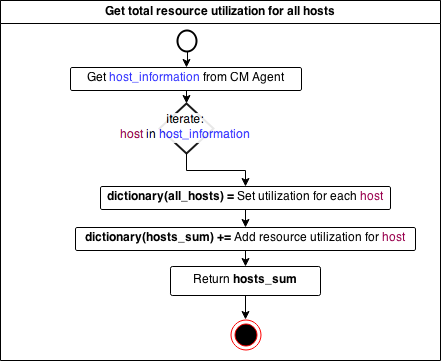
\includegraphics[width=0.6\textwidth]{images/design/cm_get_host_utilization}

\caption{Check resource utilization of hosts}
\end{figure}

The amount of resources that are required in total to deploy the topology on the tenant needs to be calculated by adding up the amount of resources that are needed for each Unit. This can easily be done by checking its flavor.

\begin{figure}[H]
\centering

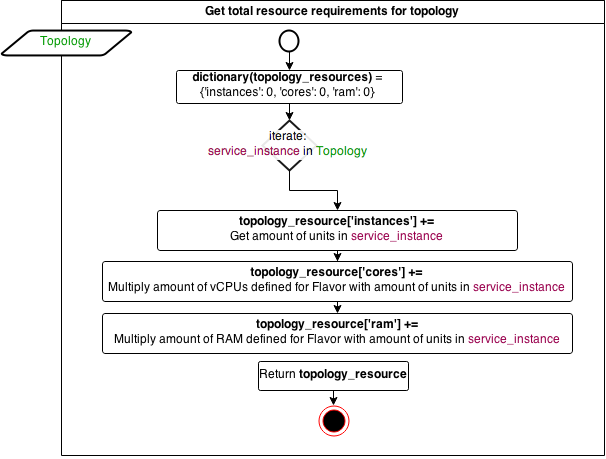
\includegraphics[width=0.6\textwidth]{images/design/cm_get_topology_requirements}

\caption{Get total amount of required resources for topology}
\end{figure}

\textbf{Step 2: Check if Topology is within the limitations of the Quota and currently available resources on the tenants hosts.}

\begin{figure}[H]
\centering

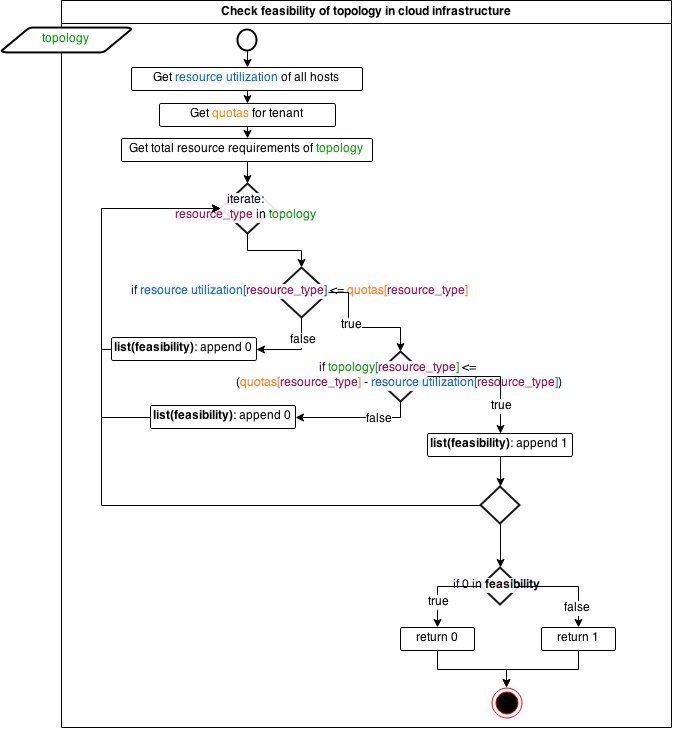
\includegraphics[width=0.7\textwidth]{images/design/cm_feasibility_check}

\caption{Deployment feasibility check}
\end{figure}


\textbf{Step 3: Check whether the Topology can be deployed on a single host.}

\begin{figure}[H]
\centering

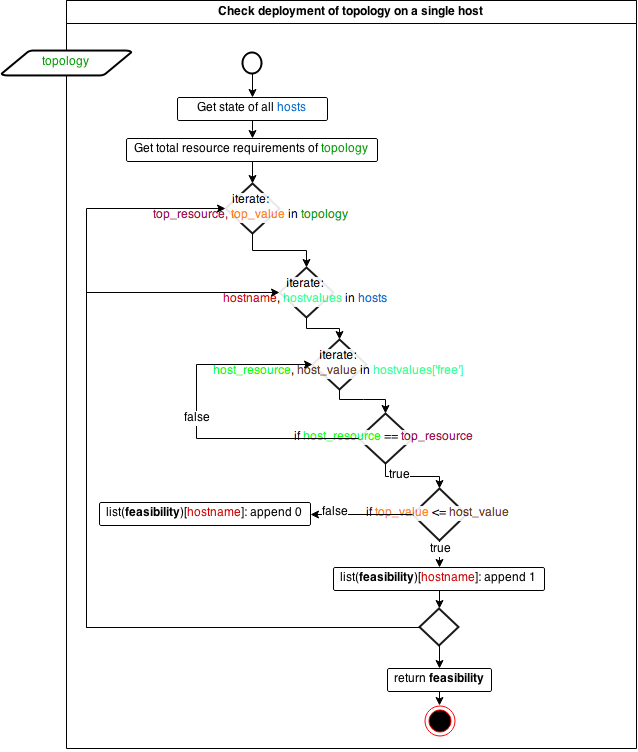
\includegraphics[width=0.7\textwidth]{images/design/cm_single_host_check}

\caption{Single host deployment check}
\end{figure}


\textbf{Step 4: Set selected host as availability zone for each Unit.}

\begin{figure}[H]
\centering

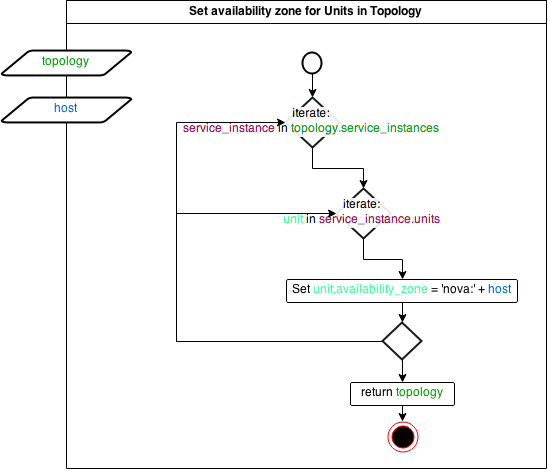
\includegraphics[width=0.7\textwidth]{images/design/cm_set_az_topology}

\caption{Set AZ per Unit}
\end{figure}

\subsubsection{Enabling QoS for VM}

.. ToDO: Mention configuration file!!

\begin{figure}[H]
\centering

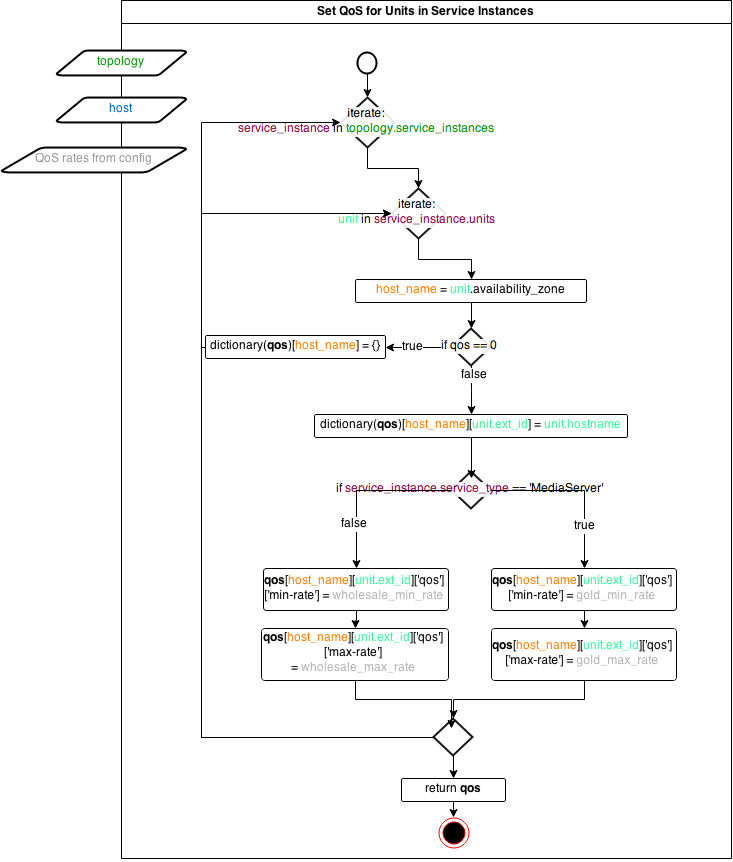
\includegraphics[width=0.5\textwidth]{images/design/cm_set_qos.png}

\caption{Method for setting QoS for all Units}
\end{figure}


\section{Connectivity Manager Agent components and operations}

\begin{figure}[H]
\centering

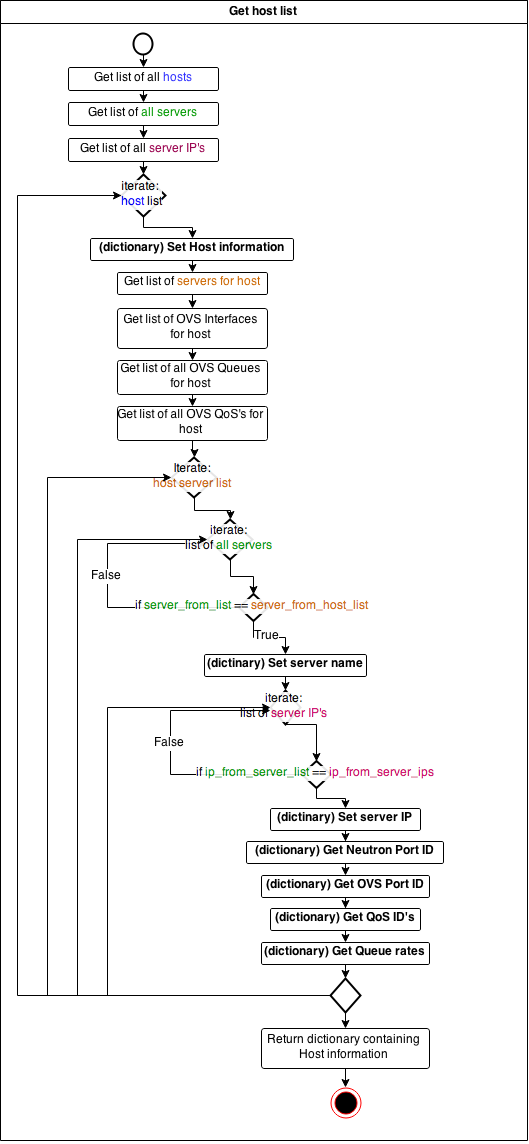
\includegraphics[width=0.7\textwidth]{images/design/activity_host_list}

\caption{Activity diagram: Get list of hosts}
\end{figure}

\begin{figure}[H]
\centering

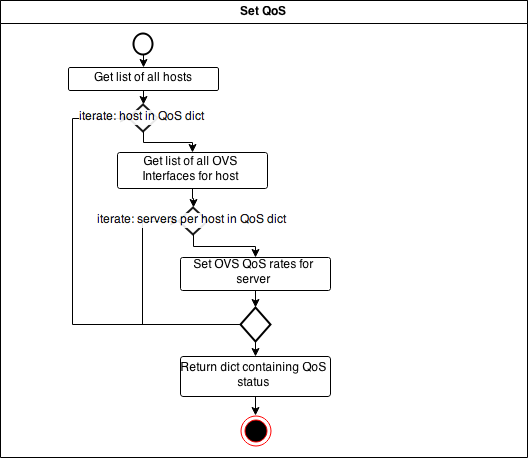
\includegraphics[width=0.7\textwidth]{images/design/activity_set_qos}

\caption{Activity diagram: Set QoS rates for all servers}
\end{figure}

\begin{figure}[H]
\centering

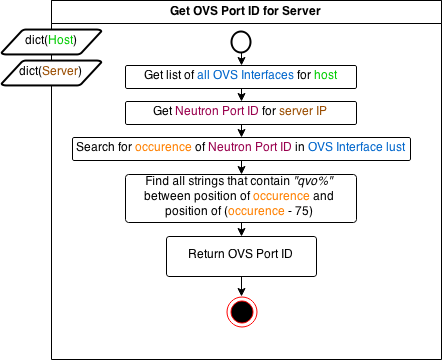
\includegraphics[width=0.7\textwidth]{images/design/activity_get_ovs_port_server}

\caption{Activity diagram: Get OVS Port ID for server}
\end{figure}

\begin{figure}[H]
\centering

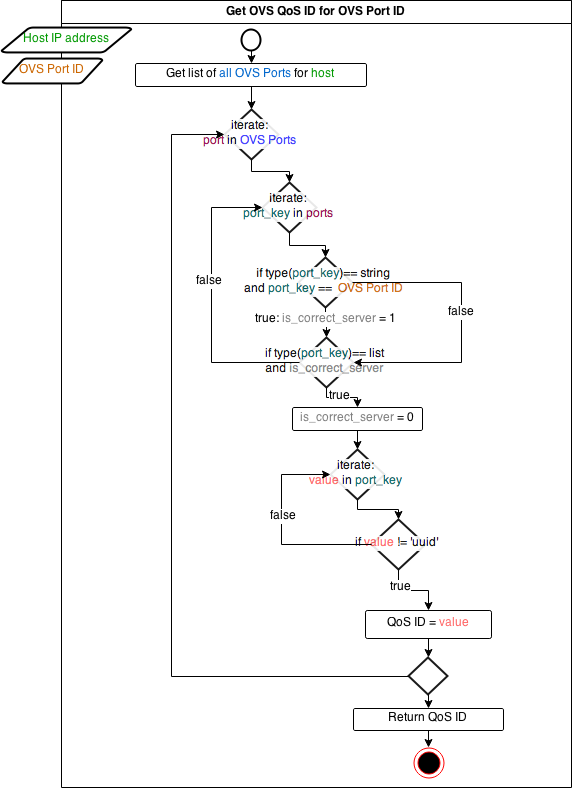
\includegraphics[width=0.7\textwidth]{images/design/activity_get_qos_id_for_ovs_port}

\caption{Activity diagram: Get QoS ID for OVS Port}
\end{figure}


\section{Conclusion}